%  Synergies and mergers-Thursday, 19 November 2020
%
%  Created by Patrick on 2020-11-19.
%  Copyright (c) 2020 __Patrick Legros__. All rights reserved.
%
%!TEX encoding = UTF-8 Unicode  

\documentclass[a4paper]{article}
\usepackage[utf8]{inputenc}
\usepackage{amsmath}
\usepackage{amssymb}
\usepackage{url}
\usepackage{hyperref}
%\usepackage[round]{natbib}
%\bibliographystyle{plainnat}
\usepackage[mathscr]{euscript}
\let\euscr\mathscr \let\mathscr\relax
\usepackage[scr]{rsfso}
\usepackage{graphicx}
\usepackage{float}
\usepackage{enumerate}
\usepackage{blindtext}
\usepackage{setspace}
\usepackage{eurosym}
\usepackage{hyperref}
\usepackage{pdflscape}
\usepackage{array, multirow}
\newcommand*{\qed}{\hfill\ensuremath{\blacksquare}}%
\usepackage[dvipsnames]{xcolor}

\usepackage{todonotes}

\usepackage{tikz}
\hypersetup{
colorlinks,
citecolor=NavyBlue,
linkcolor=NavyBlue,
urlcolor=NavyBlue}
\usetikzlibrary{matrix}
\newtheorem{prop}{Proposition}
\newtheorem{lemma}{Lemma}
\newtheorem{corollary}{Corollary}
\newtheorem{ass}{Assumption}
\newtheorem{result}{Result}
\newtheorem{condition}{Condition}
\newtheorem{Theorem}{Theorem}
\newtheorem{Definition}{Definition}

\newenvironment{reusefigure}[2][htbp]
  {\addtocounter{figure}{-1}%
   \renewcommand{\theHfigure}{dupe-fig}% If you're using hyperref
   \renewcommand{\thefigure}{\ref{#2}}% Figure counter is \ref
   \renewcommand{\addcontentsline}[3]{}% Avoid placing figure in LoF
   \begin{figure}[#1]}
  {\end{figure}}
  
  \usepackage{titlesec}

%\setcounter{secnumdepth}{4}

\titleformat{\paragraph}
{\normalfont\normalsize\bfseries}{\theparagraph}{1em}{}
\titlespacing*{\paragraph}
{0pt}{3.25ex plus 1ex minus .2ex}{1.5ex plus .2ex}

 \usepackage{geometry}

 
 \newcommand{\E}{\mathbb E}
 \newcommand{\M}{\mathcal M}
\renewcommand{\th}{\hat\theta}
\renewcommand{\t}{\theta}

\begin{document}


\title{Synergistic information$^2.0$}
\author{Antoine Dubus and Patrick Legros\thanks{We would like to thank.}}
\date{\today}

%\author{Antoine Dubus\thanks{~~Université Libre de Bruxelles, ECARES; \href{mailto:antoine1dubus@gmail.com}{antoine1dubus@gmail.com}.}}

\maketitle

\begin{abstract}

\noindent 

\end{abstract}
 
\textbf{Very preliminary, do not circulate.}

\baselineskip0.7cm

\section{Literature}
\begin{itemize}\setlength\itemsep{-1em}
    \item Optimal merger policy when firms have private information \cite{Besanko1993}
    \item Information sharing in oligopolies
    \item Data as assets
    \item Computer science and data synergies
    \item Joint ventures before merger
\end{itemize}

\section{Model}


\begin{itemize}\setlength\itemsep{0em}
	\item Two firms, 1 and 2. 
	\item Firm $1$ is endowed with a data set $X$. Firms make profits using data. 
	\item The firms may eventually to merge but can engage in data sharing. Data sharing involves a transaction of an amount of data $s\leq X$ at price $T(s)$ paid by firm $2$ to firm $1$. This price can be equal to zero in the case of voluntary sharing (may also be relevant when the two firms have datasets.)
	\item The amount of data that is shared is verifiable, in particular by the regulator. 
	\item The regulator will choose whether to allow the merger or not. The regulator tradeoffs the cost from increased market power (assumed to simplify to be proportional to the industry profit) and the gain from having the two firms have similar data $\t B(s)$, with $B$ increasing and concave, and $\t$ having distribution $F(\t)$ on $[0,\infty)$. We will assume that (perhaps too early to put this assumption)
	 %
   \begin{equation}\label{ass:B}
       B(X)>X \text{ and } B(0)=0.
   \end{equation}
    %
	\item If there is no merger, the information that has been shared by Firm $1$ can be used by Firm 2 during the competition, and information sharing changes the profit of Firm $1$: $X-\t l s$; and of Firm 2: $\t s$. Hence the total industry profit if there is competition is $X-\t s(1-l)$. The model nests two interpretations:
\begin{enumerate}[(a)]
    \item (Costly Sharing:) $l\geq 0$: sharing information increases competition and firm $1$ incurs a loss that is increasing in the amount that is shared.
    \item (Collusive Sharing:) $l< 0$: sharing information facilitates coordination and increases the profits of a firm (à la \cite{vives1984duopoly} for instance) in an increasing way $s$.
 \end{enumerate}
    \item After $s$ is shared and $T(s)$ is sunk, firm $2$ learns the value of $\t$ and both firms can agree to approach the regulator to ask for their merger to be approved. 
    
\end{itemize}

\paragraph{The timing of the game is the following.} 
\begin{enumerate}\setlength\itemsep{0em}
    \item Firms $1,2$ agree on a sharing of data together with a price for the transaction. At this stage, firm $1$ may have private information about the benefit to firm $2$ of the data that is shared. 
    \item If $s>0$ is shared, firm $2$ learns the true value of $\t$, and the firms decide to merge and approach the regulator.
    \item The regulator knows $s$ and decides whether to allow the merger. If the merger is approved, the regulator anticipates that the merged entity will bring a social benefit of $\t B(X)$ and the industry will make profit $\pi^m(s)=X(1+\t)$ (the regulator does not know however the realization of $\t$). If the merger is not approved, the regulator anticipates a benefit of $\t B(s)$ for an industry profit of $X+\t s(1-l)$.
\end{enumerate}
%
\subsection{The Regulator's Problem}
   The regulator maximizes a social welfare function that weights the social cost of high industry profits and the social benefit of synergies. Contrary to the usual view that synergies are created only during the merger, synergies endogenously happen without a merger if firm $1$ shares some of its data with firm $2$. Hence, when evaluating a merger proposal, the regulator will compare the \emph{relative synergy gain} $\t (B(X)-B(s))$ to the \emph{relative industry profit gain.} $X(1+\t)-(X+\t s(1-l))$. Our specification yields  the desirable simplification that this comparison is independent of the realization of $\t$. This allows us to focus on the problem, similar to \cite{anton2002sale}, of firm $1$ convincing firm $2$ to pay a high price for data. Nevertheless the regulator plays a non-trivial role because the amount of sharing will affect the likelihood of the regulator authorizing the merger. 

   The condition for authorizing the merger is 
   %
   \[
   B(X)-X\geq B(s)-s(1-l).
   \]
   %
By concavity of $B(s)$, the function $B(s)-s(1-l)$ is concave in $s$. Figure \ref{fig:l<0} illustrates, when sharing is costly, a sitautions where the regulator authorizes the merger only for $s$ is smaller than $\underline s>0$ or greater than $\overline s\in(\underline s,X]$. If $B(X)-X$ is greater than $B(s)-s(1-l)$, the regulator authorizes the merger for any value of $s$. 

If sharing is collusive, that is $l<0$, the curve $B(s)-s(1_l)$ is everywhere above $B(s)-s$, and therefore, the regulator is more reluctant to authorize a merge: he will do so when $s$ is less than a bound $\underline s(l)$ that is a decreasing function of $l$. Hence, the more collusive information sharing is, the less likely is a merger accepted.

\begin{figure}[h!]
    \centering
    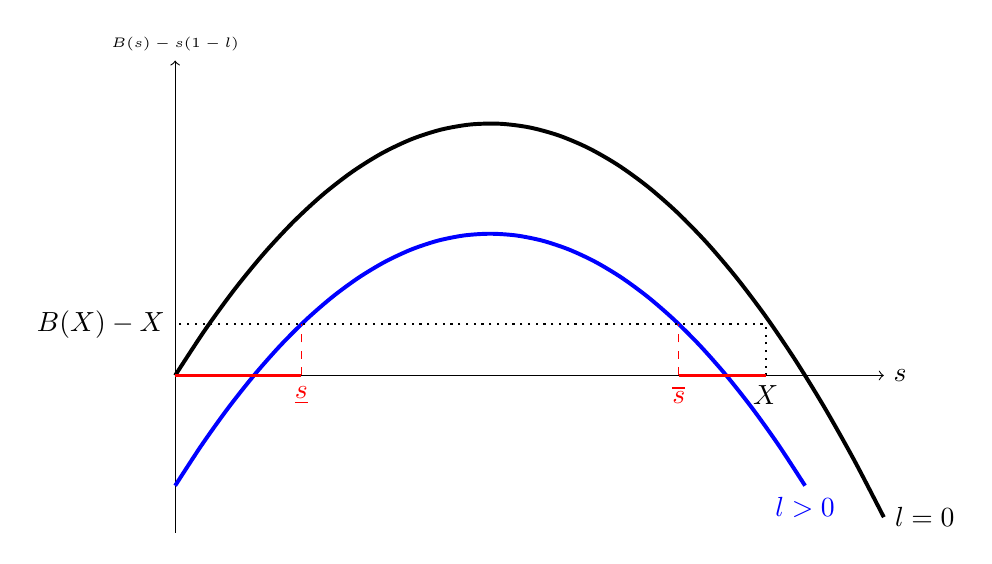
\begin{tikzpicture}
        \draw[->] (0,0)--(9,0) node[right]{$s$};
        \draw[->] (0,-2)--(0,4) node[above]{\tiny$B(s)-s(1-l)$};
        \draw[black, line width = 0.50mm]   plot[smooth,domain=0:9] (\x, {\x*(8-\x)/5}) node[right]{$l=0$};
        \draw[blue, line width = 0.50mm]   plot[smooth,domain=0:8] (\x, {(\x-1)*(7-\x)/5}) node[below]{$l>0$};
        \draw[dotted, thick] (7.5,0)node[below]{$X$}--(7.5,0.65) -- (0,0.65)node[left]{$B(X)-X$};
        \draw[red,very thick] (1.60208,0)node[below]{$\underline s$}--(0,0);
        \draw[red,very thick] (6.39792,0)node[below]{$\overline s$}--(7.5,0);
            \draw[dashed,red] (1.60208,0)--((1.60208,0.65) (6.39792,0) --(6.39792,0.65);
    \end{tikzpicture}
    \caption{Costly sharing ($l>0$)}
    \label{fig:l>0}
\end{figure}


\section{Playing the Regulatory Game with Costly Sharing: Perfect Information and Costly Sharing}
Suppose that at period $1$, both firms know $\theta$. We proceed by backward inducation. Fix $\t$ and let $(s,T)$ be the agreed upon sharing and price at the first period. The total surplus is $X+\t s(1-l)$ and therefore, the optimal sharing is $s=0$ if $l> 1$ and is $s=X$ if $l<1$. 

If $l>1$, the optimal sharing when firms ignore the possibility of a merge is to use $s=0$. Given this sharing, the regulator will accept the merger.  

Suppose that $l<1$. Because $s=X$, the merger is not authorized. Therefore, the profits of firms $1,2$ are respectively $X(1-\t l)+T,\t X -T$. The alternative is for the firms not to share, in which case \emph{the merger is approved}, and firms get some share of the total surplus $X(1+\t)$. 


\bibliographystyle{plain}
\bibliography{Bibliography}





\end{document}

